\begin{figure}
    \begin{center}
    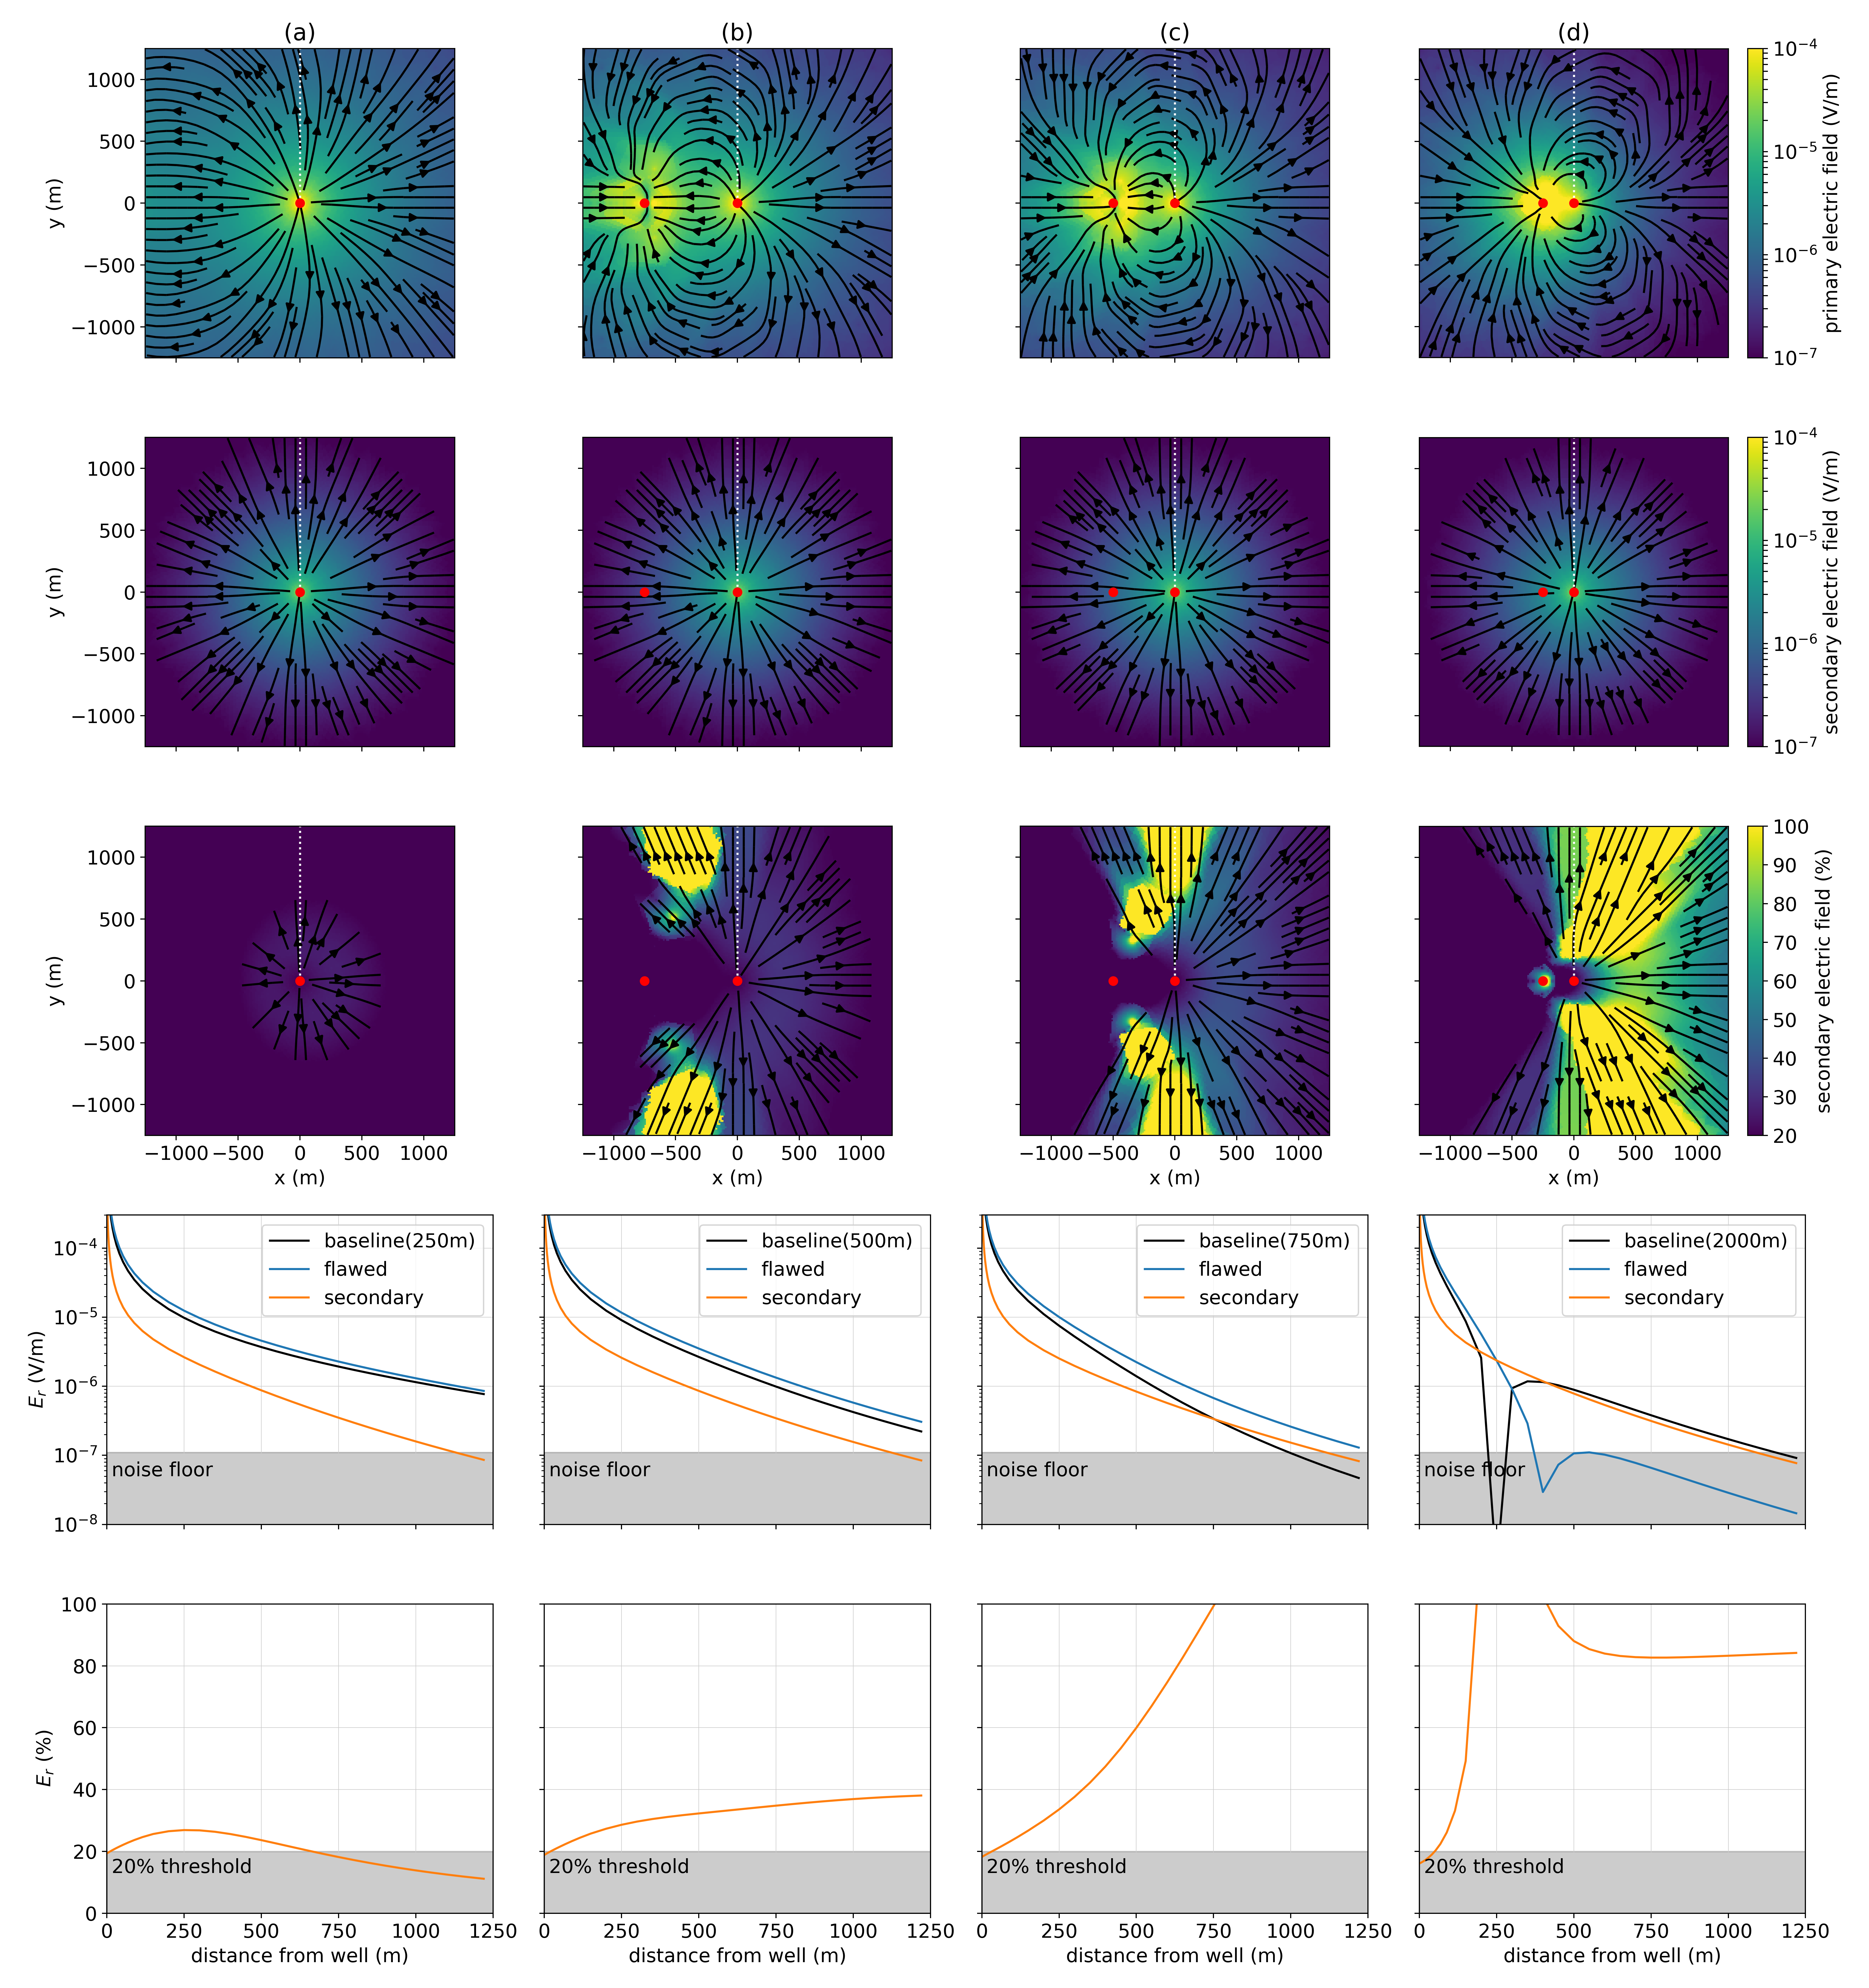
\includegraphics[width=\textwidth]{figures/dc_casing/integrity_e_fields.png}
    \end{center}
\caption{
    (Top row) primary electric field, (second row) secondary electric field,
    and (third row) secondary electric field as a percentage of the primary radial electric field
    for a return electrode that is offset (a) 2000m, (b) 750m, (c) 500m, and (d) 250m
    from the well. The primary is defined as the response due to the 1000m
    long, intact well. In each figure, the electrode locations are denoted by
    the red dots. In the third row, the colorbar has been limited
    between 20\% and 100\%. The fourth and fifth rows show radial electric field data
    collected along the $\theta=90^\circ$ azimuth (the white dotted lines in
    the top three rows). The fourth row shows the primary (black line), the total
    electric field due to the flawed well (blue line), and the secondary
    radial electric field (orange line). The fifth row shows the secondary as a
    percentage of the primary.
}
\label{fig:integrity_e_fields}
\end{figure}
